\begin{frame}\begin{center}
{\LARGE\textbf{Paper}}
\end{center}\end{frame}
%-------------------------------------------------------------------------------
%-------------------------------------------------------------------------------
\begin{frame}
\begin{quote}\small
This paper formulates and estimates multistage production functions for children cognitive and noncognitive skills. Skills are determined by parental environments and investments at different stages of childhood. We estimate the elasticity of substitution between investments in one period and stocks of skills in that period to assess benefits of early investment in children compared to later remediation. $\hdots$ Using the estimated technology, we determine optimal targeting of interventions to children with different parental and personal birth endowments. $\hdots$
\end{quote}
\end{frame}
%-------------------------------------------------------------------------------
%-------------------------------------------------------------------------------
\begin{frame}
\begin{itemize}
\item\bibentry{Cunha.2010}
\end{itemize}\vspace{0.3cm}

Part of a whole sequence ...\vspace{0.3cm}

{\scriptsize\begin{itemize}
\item\bibentry{Cunha.2007}
\item\bibentry{Cunha.2008c}
\end{itemize}}\vspace{0.3cm}

\end{frame}

%-------------------------------------------------------------------------------
%-------------------------------------------------------------------------------
\begin{frame}
\textbf{Model}
\begin{align*}\begin{array}{ll}
t\in\{1, 2, \hdots, T\} & \text{childhood periods} \\
s\in\{1, \hdots, S\}    & \text{developmental stages}  \\
k \in\{C, N\}          & \text{skill type} \\
\theta_{k,t}           & \text{level of skill} \\
I_{k,t}                 & \text{parental investment} \\
\end{array}\end{align*}
\end{frame}
%-------------------------------------------------------------------------------
%-------------------------------------------------------------------------------
\begin{frame}
The technology of production of skill $k$ in period $t$ and developmental stage $s$ depends on the stock of skills in period $t$, investment at $t$, $I_{k,t}$, parental skills, $\theta_P$, shocks in period $t$, $\eta_{k, t}$, and the
production function at stage $s$.

\begin{align*}
\theta_{k, t + 1} = f_{k, s}(\theta_t, I_{k, t}, \theta_P, \eta_{k, t}), \\
\end{align*}
where $k\in\{C, N\}$, $t\in\{1, \hdots, T\}$, and $s\in\{1, \hdots, S\}$.

\end{frame}
%-------------------------------------------------------------------------------
%-------------------------------------------------------------------------------
\begin{frame}\textbf{Direct Complementarity}

\begin{align*}
\frac{\partial^2 f_{k, s}(\cdot)}{\partial I_{k, t}\partial \theta_{l, t}} > 0, \qquad\text{where}\;t\in\{1,\hdots,T\}, \; l,k\in\{C, N\}
\end{align*}

Period $t$ stocks of abilities and skills promote the acquisition of skills by making investment more productive.

\end{frame}
%-------------------------------------------------------------------------------
%-------------------------------------------------------------------------------
\begin{frame}\begin{figure}\caption{Optimal Investment Ratios}
\scalebox{0.75}{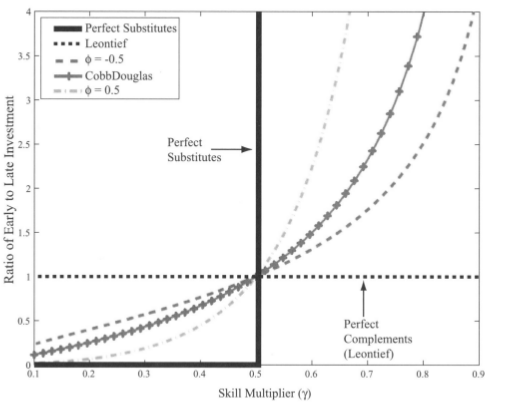
\includegraphics{material/fig-early-late}}
\end{figure}\end{frame}
%-------------------------------------------------------------------------------
%-------------------------------------------------------------------------------
\begin{frame}\textbf{Adult Outcomes}\vspace{0.3cm}

Adult outcome $j$, $Q_j$, is produced by a combination of different skills at the beginning of period $T + 1$.
\begin{align*}
Q_j = g_j(\theta_{C, T + 1}, \theta_{N, T + 1}), \qquad j \in\{1, \hdots, J\}
\end{align*}

\end{frame}
%-------------------------------------------------------------------------------
%-------------------------------------------------------------------------------
\begin{frame}\textbf{Technology Equation}\vspace{0.3cm}

\begin{align*}
\theta_{k, t + 1} & = [\gamma_{s, k, 1} \theta^{\phi_{s, k}}_{C, t}  + \gamma_{s, k, 2} \theta^{\phi_{s, k}}_{N, t}  \\
                  &  + \gamma_{s, k, 3} I^{\phi_{s, k}}_{t} +  \gamma_{s, k, 4} \theta^{\phi_{s, k}}_{C, P} + \gamma_{s, k, 5} \theta^{\phi_{s, k}}_{N, P}]^{1/\sigma_{s, k}}e^{\eta_{n, k, t +1}},
\end{align*}
where $\gamma_{s, k, l}\geq 0$, $\sum^5_{l = 1} \gamma_{s, l, k} = 1$, $k\in\{C, N\}$, $t\in\{1, 2\}$, $s\in\{1, 2\}$, and $\eta_{k,t}\sim\N(0, \sigma^2_{\eta, s})$.
\end{frame}
%-------------------------------------------------------------------------------
%-------------------------------------------------------------------------------
\begin{frame}\textbf{Measurement Equation}\vspace{0.3cm}

\begin{align*}
Z_{1, k, t, j} & = \mu_{1, k, t, j} + \alpha_{1, k, t, j}\ln\theta_{k, t} + \epsilon_{1, k, t, j} \\
Z_{2, k, t, j} & = \mu_{2, k, t, j} + \alpha_{2, k, t, j}I_{k, t} + \epsilon_{2, k, t, j}, \\
\end{align*}

where $E(\epsilon_{a, k, t, j}) = 0$, $j \in\{1,\hdots, M_{a, k, t}\}$, $t\in\{1, \hdots, T\}$, $k \in\{C, N\}$, $a\in\{1, 2\}$ and where $\epsilon_{a, k, t, j}$ are uncorrelated across the $j$.

\end{frame}
%-------------------------------------------------------------------------------
%-------------------------------------------------------------------------------
\begin{frame} 
	\small{We estimate the technology on a sample of 2,207 firstborn white children from the Children of the NLSY79 (CNLSY79) sample. Starting in 1986, the children of the NLSY97 female respondents, ages 0-14, have been assessed every 2 years. The assessments measure cognitive ability, temperament, motor and social development, behavior problems, and self-competence of the children as well as their home environments. Data are collected via direct assessment and maternal report during home visits at every biannually.}
\end{frame}
%-------------------------------------------------------------------------------
%-------------------------------------------------------------------------------
\begin{frame}\begin{figure}\caption{Signal and Noise for Skills}\vspace{-0.6cm}
\scalebox{0.60}{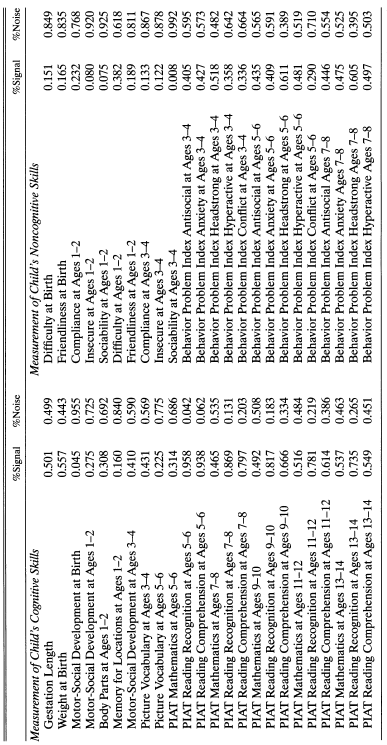
\includegraphics[angle=270]{material/fig-signal-noise-1}}
\end{figure}\end{frame}
%-------------------------------------------------------------------------------
%-------------------------------------------------------------------------------
\begin{frame}\begin{figure}\caption{Signal and Noise for Investment}\vspace{-0.6cm}
\scalebox{0.60}{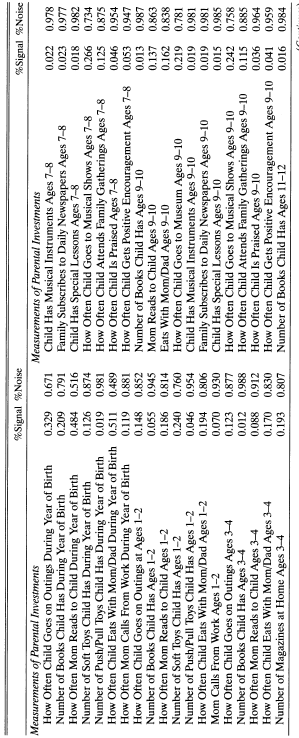
\includegraphics[angle=270]{material/fig-signal-noise-2}}
\end{figure}\end{frame}
%-------------------------------------------------------------------------------
%-------------------------------------------------------------------------------
\begin{frame}\begin{figure}\caption{Baseline Estimates}\vspace{0.3cm}
\scalebox{0.50}{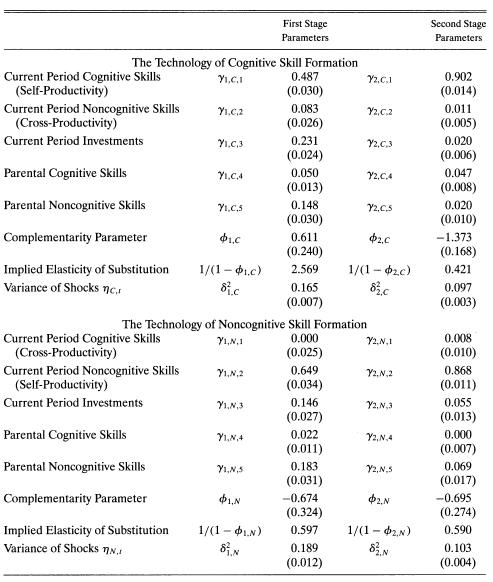
\includegraphics{material/fig-estimates-1}}
\end{figure}\end{frame}
%-------------------------------------------------------------------------------
%-------------------------------------------------------------------------------
\begin{frame}\textbf{Usefulness of Structural Models}\vspace{0.3cm}

\begin{itemize}\setlength\itemsep{1em}
\item assess relative importance of competing economic mechanisms
\item conduct ex ante policy evaluation
\end{itemize}\vspace{0.5cm}

See \citeA{Wolpin.2013} and \citeA{Rust.2014} for an instructive discussion of the usefulness and limits of structural econometric methods.

\end{frame}
%-------------------------------------------------------------------------------
%-------------------------------------------------------------------------------
\begin{frame}\textbf{Heterogeneity in Educational Attainment}\vspace{0.3cm}
\begin{itemize}\setlength\itemsep{1em}
\item 34\% skills\medskip
\begin{itemize}\setlength\itemsep{1em}
\item 16\% cognitive
\item 12\% noncognitive
\end{itemize}
\item 15\% parental investment
\end{itemize}
\end{frame}
%-------------------------------------------------------------------------------
%-------------------------------------------------------------------------------
\begin{frame}\textbf{Policy Evaluation}

\begin{align*}\begin{array}{ll}
h\in\{1\hdots, H\} & \text{children} \\
\theta_{1,h}   & \text{initial condition}  \\
S_h            & \text{schooling attainment} \\
B = 2H          & \text{budget}
\end{array}\end{align*}

\end{frame}
%-------------------------------------------------------------------------------
%-------------------------------------------------------------------------------
\begin{frame}\textbf{Optimization Problem}

\begin{align*}
\max \bar{S} & = \frac{1}{H}\sum_{h\in H} S_h(\theta_{C,3,h}, \theta_{N,3,h}) \\
s.t. & \\
     &  \sum_{h\in H} (I_{1, h} + I_{2,h}) = 2H \\
     & \theta_{k, t + 1, h} = f_{k, t}(\theta_{C,t,h}, \theta_{N,t,h}, \theta_{C, P}, \theta_{N, P})\\
     & \qquad \text{for}\quad k \in\{C, N\}\quad\text{and}\quad t\in\{1, 2\}
\end{align*}

There is an analogous constraint minimization problem for crime.

\end{frame}
%-------------------------------------------------------------------------------
%-------------------------------------------------------------------------------
\begin{frame}\begin{figure}\caption{Aggregate Education by Initial Conditions}\vspace{0.3cm}
\scalebox{0.60}{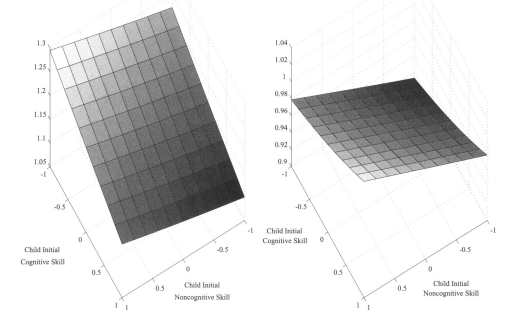
\includegraphics{material/fig-optimal-policy-1}}
\end{figure}\end{frame}
%-------------------------------------------------------------------------------
%-------------------------------------------------------------------------------
\begin{frame}\begin{figure}\caption{Aggregate Education by Maternal Endowment}\vspace{0.3cm}
\scalebox{0.80}{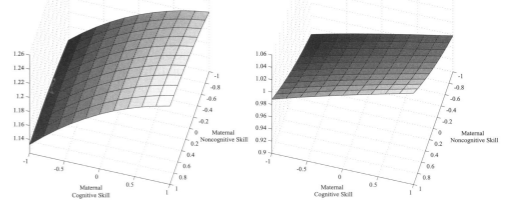
\includegraphics{material/fig-optimal-policy-2}}
\end{figure}\end{frame}
%-------------------------------------------------------------------------------
%-------------------------------------------------------------------------------
\begin{frame}\begin{figure}\caption{Aggregate Crime by Initial Conditions}\vspace{0.3cm}
\scalebox{0.80}{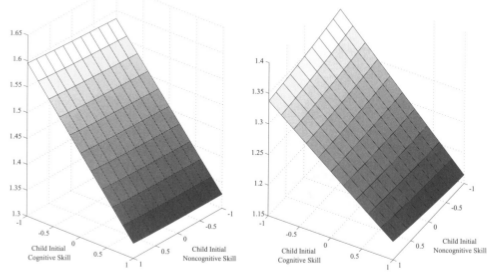
\includegraphics{material/fig-optimal-policy-3}}
\end{figure}\end{frame}
%-------------------------------------------------------------------------------
%-------------------------------------------------------------------------------
\begin{frame}\begin{figure}\caption{Aggregate Crime by Maternal Endowment}\vspace{0.3cm}
\scalebox{0.80}{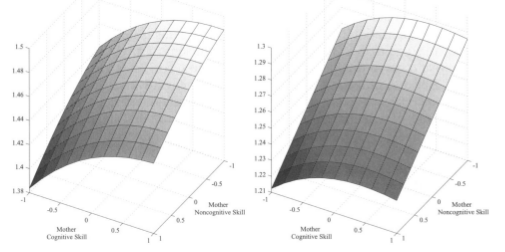
\includegraphics{material/fig-optimal-policy-4}}
\end{figure}\end{frame}
%-------------------------------------------------------------------------------
%-------------------------------------------------------------------------------
\begin{frame}\begin{figure}\caption{Density Ratios}\vspace{0.3cm}
\scalebox{0.80}{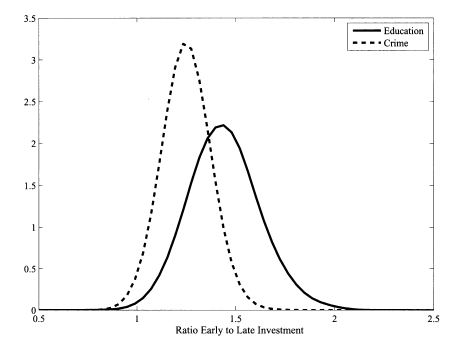
\includegraphics{material/fig-optimal-policy-5}}
\end{figure}\end{frame}
%-------------------------------------------------------------------------------
%-------------------------------------------------------------------------------
\begin{frame}
\begin{quote}
These simulations suggest that the timing and level of optimal interventions for disadvantaged children depend on the condition for disadvantage and the nature of desired outcomes. Targeted strategies are likely to be effective especially for different targets that weight cognitive and noncognitive skills differently.
\end{quote}
\end{frame}
%-------------------------------------------------------------------------------
%-------------------------------------------------------------------------------
\begin{frame}\textbf{Key Contributions}\vspace{0.3cm}

\begin{itemize}\setlength\itemsep{1em}
\item formulation and estimation of a multistage model with multidimensional skills
\item illustration of the importance of distinguishing between early and late investments
\item nonparametric identification of production technology
\end{itemize}\vspace{0.3cm}

What is next?

\end{frame}
%-------------------------------------------------------------------------------
%-------------------------------------------------------------------------------
